\documentclass[a4paper,14pt]{report}
\usepackage{tikz}
\usepackage[utf8]{inputenc}
\usepackage[russian]{babel}
\usepackage{amsmath}
\usepackage{listings}
\usepackage{pdfpages}
\lstset{ 
	extendedchars=\true,
	stringstyle=\bf,
	commentstyle=\textit,
	language=C++, % choose the language of the code
	basicstyle=\ttfamily,
	keywordstyle=\color{black}\bfseries, % style for keywords
	numbers=none, % where to put the line-numbers
	numberstyle=\tiny, % the size of the fonts that are used for the line-numbers     
	backgroundcolor=\color{lightgray},
	showspaces=false, % show spaces adding particular underscores
	showstringspaces=false, % underline spaces within strings
	showtabs=false, % show tabs within strings adding particular underscores
	frame=single, % adds a frame around the code
	tabsize=2, % sets default tabsize to 2 spaces
	%rulesepcolor=\color{gray}
	captionpos=t, % sets the caption-position to bottom
	breaklines=true, % sets automatic line breaking
	breakatwhitespace=false 
}
\usetikzlibrary{calc, matrix}

%{{{Command defns
\newcommand{\definition}[2]
{
	\textbf{#1} -- #2\\
}
\newlength{\drop}
\newcommand*{\titleMS}{\begingroup
	\centering
	\includegraphics[height=2.0cm, width=2.0cm]{mirea.png}\\
	{\sffamily МИНОБРНАУКИ РОССИИ}\par
	\hbox to 40pt{\hfil\bfseries Федеральное государственное бюджетное образовательное учреждение\hfil}\par
	{\bfseries высшего профессионального образования}\par
	\hbox to 40pt{\hfil\bfseries "Московский государственный технический университет радиотехники,\hfil}\par
	{\bfseries электроники и автоматики"}\par
	\vspace{1.5pt}
	{\LARGE\bfseries МГТУ МИРЭА}\\[-0.5cm]
	\linethickness{1.8mm}
	\begin{flushleft}
		\line(1,0){410}\par
	\end{flushleft}
	\linethickness{0.2mm}
	\vbox {
	Кибернетика\\[-0.35cm]
	\line(1,0){300}\\[-0.1cm]
	{\it (наименование факультета)}\par
	\vspace{1.5pt}
	}
	Прикладная математика и информатика\\[-0.35cm]
	\line(1,0){300}\\[-0.1cm]
	{\it (наименование кафедры)}\par
	\vspace{0.3in}
	{\LARGE\bfseries КУРСОВАЯ РАБОТА}\par
	\vspace{1.5pt}
	{\LARGE\bfseries по дисциплине}\par
	{\large <<Численные методы>>}\\[-0.35cm]
	\line(1,0){300}\\[-0.1cm]
	{\it (наименование дисциплины)}\par
	\vspace{1.5pt}
	{\large\bfseries Тема курсовой работы}\\
	Построение аппроксимирующей функции методом Паде\\[-0.35cm]
	\line(1,0){300}\\
	\line(1,0){300}\\
	\vspace{0.5in}
	\begin{tabular}{|p{2.5in}| c |}
		\hline
		Студент группы КБ-32-10& Дорофеев А.Н.\\[-0.4cm] &\line(1,0){200}\\
		&\small{\it{(Фамилия И.О.)}}\\
		\hline
		Руководитель курсовой работы & Строганов А.\\[-0.4cm] &\line(1,0){200}\\
		 &\small{\it{(Фамилия И.О.)}}\\
		\hline
		Рецензент\it{(при наличии)} & \line(1,0){200} \\
		  &\small{\it{(Фамилия И.О.)}}\\
		\hline
	\end{tabular}\par
	\vspace{0.1in}
	\begin{tabular}{p{2.3in} p{2in} p{2in}}
		Работа представлена к защите&<<\line(1,0){15}>>\line(1,0){60}201\line(1,0){15}г.&\line(1,0){100}\\
			&&\small{\it{(подпись студента)}}\\
		<<Допущен к защите>>&<<\line(1,0){15}>>\line(1,0){60}201\line(1,0){15}г.&\line(1,0){100}\\
			&&\small{\it{(подпись руководителя)}}\\
	\end{tabular}\hfill
\endgroup}
%}}} 

\begin{document}
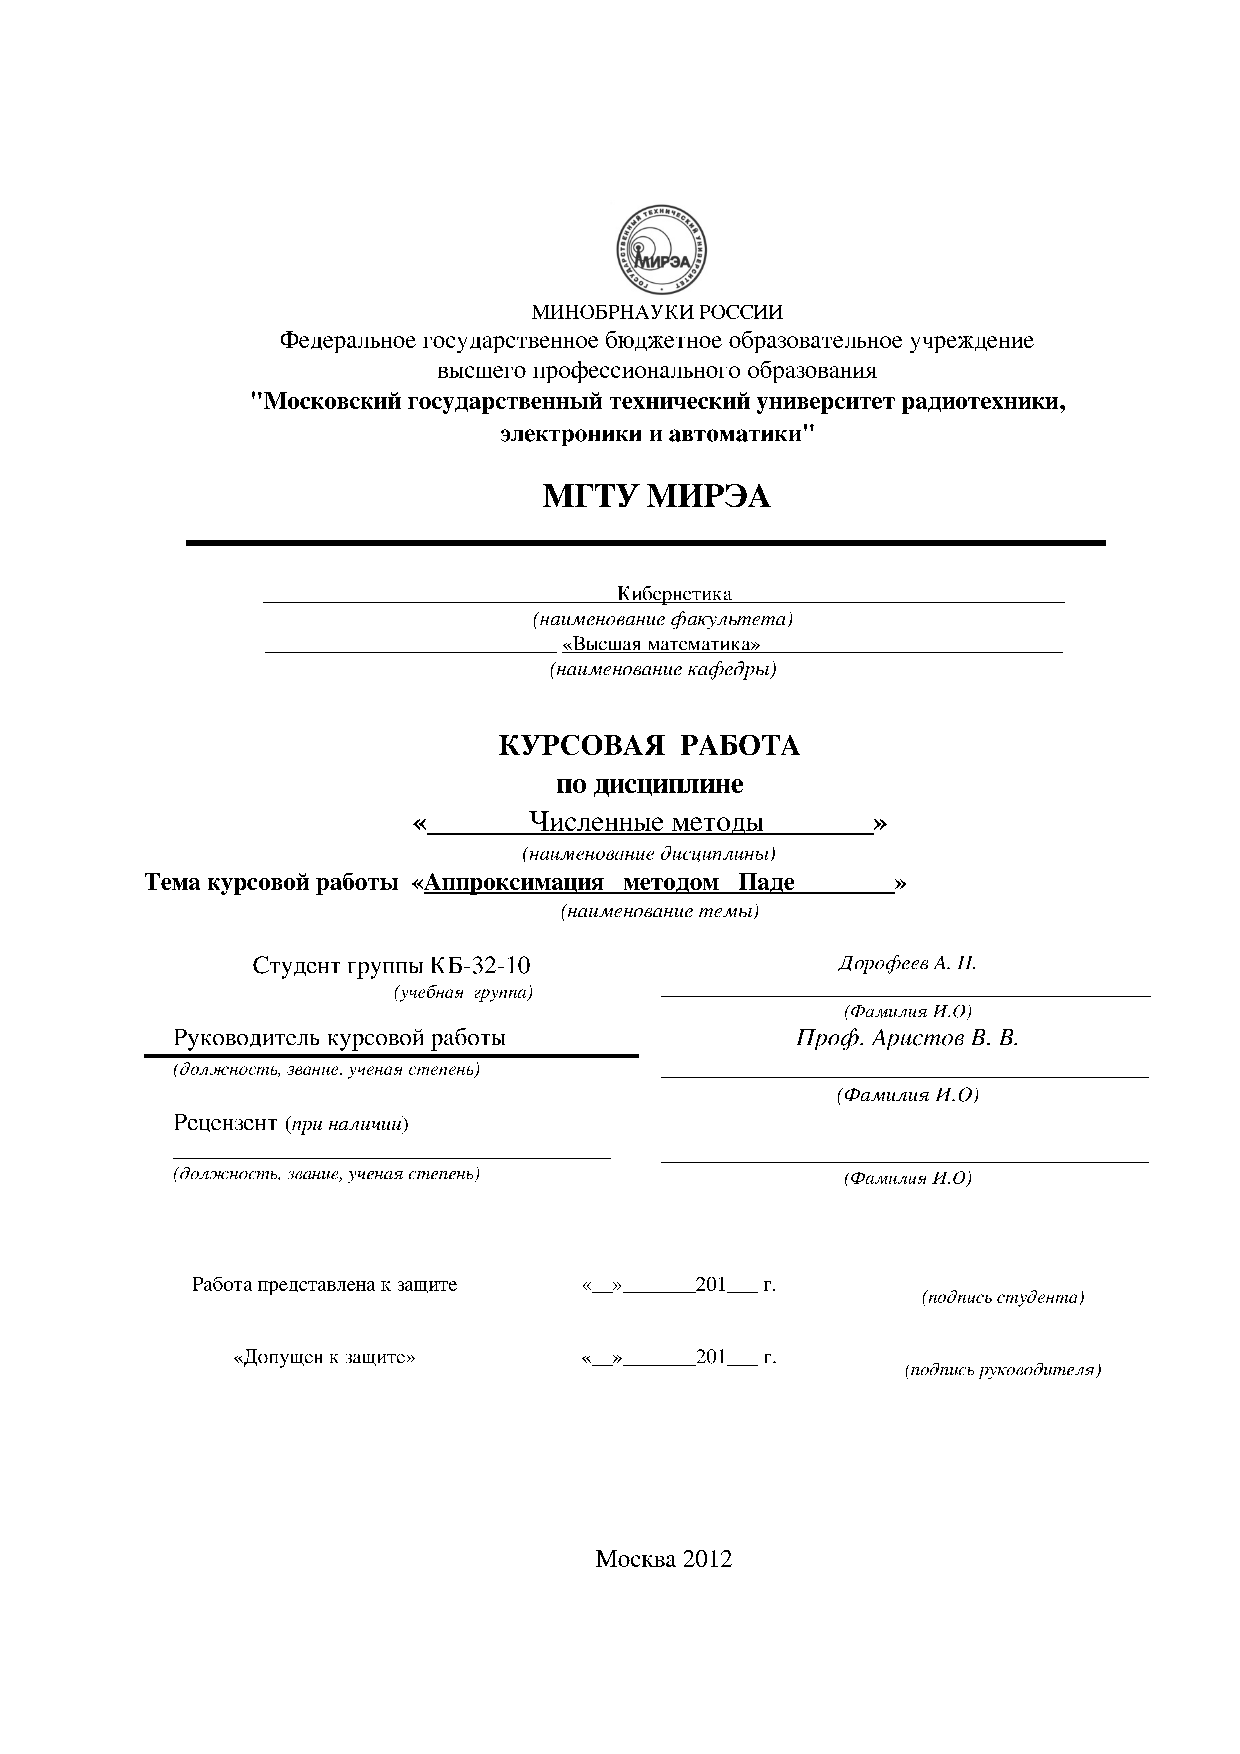
\includepdf[pages={1}]{titulniy.pdf}
\tableofcontents
\newpage
\section*{Понятия и определения} % (fold)%{{{
\addcontentsline{toc}{section}{Понятия и определения}
\definition{Рациональная функция}{дробь, числителем и знаменателем которой являются многочлены}
\definition{Аппроксимация (приближение)}{научный метод, состоящий в замене одних объектов другими, 
в том или ином смысле близкими к исходным, но более простыми}
%}}} 
\section*{Постановка задачи} % (fold)%{{{
\addcontentsline{toc}{section}{Постановка задачи}
Требуется написать программу, строящую по коэффициентам разложения 
исходной функции в ряд Маклорена её приближение рациональной функцией
методом Паде и выводящую результат в формате $\TeX$.
%}}}
\section*{Входные данные} %{{{
\addcontentsline{toc}{section}{Входные данные}
Коэффициенты разложения в ряд Маклорена исходной функции, записанные подряд с пробелами в качестве 
разделителей в файле input.dat, находящемся
в одном каталоге с исполняемым файлом.
%}}}
\section*{Выходные данные} %{{{
\addcontentsline{toc}{section}{Выходные данные}
Список коэффициентов в stdout и \TeX-файл, содержащий искомую дробно-рациональную функцию.
%}}}
\section*{Описание метода} % (fold)%{{{
\addcontentsline{toc}{section}{Описание метода}
Исходная функция $f(x)$ представляется своим рядом Тейлора:\\
\[
	f(x) = c_0 + c_1x + c_2x^2 + ... + c_kx^k
\]
Приближающая функция с многочленом степени $L$ в числителе и $M$ в знаменателе обозначается 
$R_{[L/M]}(x)$ и выглядит следующим образом: 
\[
	R_{[L/M]}(x) = 
	\frac{a_0 + a_1x + a_2x^2 + ... + a_Lx^L}
		{b_0 + b_1x + b_2x^2 + ... + b_Mx^M}
\]

$b_0$ в знаменателе можно заменить на 1 не нарушая общности, тем самым сократив количество коэффициентов:
\[
	R_{[L/M]}(x) = 
	\frac{a_0 + a_1x + a_2x^2 + ... + a_Lx^L}
		{1 + b_1x + b_2x^2 + ... + b_Mx^M}
	\]
	Далее:
	\begin{gather*}
			f(x) = R(x) \nonumber \\
			\frac{a_0 + a_1x + a_2x^2 + ... + a_Lx^L}
			{1 + b_1x + b_2x^2 + ... + b_Mx^M} = 
			c_0 + c_1x + c_2x^2 + ... + c_kx^k \nonumber \\
			a_0 + a_1x + a_2x^2 + ... + a_Lx^L = 
			(c_0 + c_1x + c_2x^2 + ... + c_kx^k)
			(1 + b_1x + b_2x^2 + ... + b_Mx^M) \nonumber
	\end{gather*}

последнее равенство эквивалентно системе уравнений:\\
\[
	\left\{
		\begin{array}{l}
			a_0 = c_0\\ 
			a_1 = c_0b_1 + c_1\\
			a_2 = c_0b_2 + c_1b_1 + c_2\\
			\ldots\\
			a_L = c_0b_L + c_1b_{L-1} + ... + c_L\\
			0 = b_Mc_{L-M+1} + b_{M-1}c_{L-M+2} + ... + b_1c_L + c_{L+1}\\
			\ldots\\
			0 = b_Mc_L + b_{M-1}c_{L+1} + ... + b_1c_{L+M-1} + c_{L+M}
		\end{array}
		\right. \\
	\]
Здесь $b_i, i>M$ может быть неопределен, если $L>M$. В этом случае просто 
положим такие $b_i$ равными нулю.

Перепишем систему так, чтобы неизвестные оказались слева:
\[
	\left\{
		\begin{array}{l}
			a_0 = c_0\\ 
			a_1 - c_0b_1 = c_1\\
			a_2 - c_1b_1 - c_0b_2 = c_2\\
			\ldots\\
			a_L - b_1c_{L-1} - b_2c_{L-2} - ... - b_Lc_0=  c_L\\
			- b_1c_L - b_2c_{L-1} - ... - b_Lc_1 = c_{L+1}\\
			\ldots\\
			- b_1c_{L+M-1} - b_2c_{L+M-1} - ... - b_Mc_{L} = c_{L+M} 
		\end{array}
		\right. \\
	\]

Системам соответствует матрица:
$$
	\begin{pmatrix}
		1	&	0	&	0	&	0	&	\ldots	&	0	&	0	&	0	&	\ldots	&	0	\\
		0	&	1	&	0	&	0	&	\ldots	&	0	&	-c_0	&	0	&	\ldots	&	0	\\
		0	&	0	&	1	&	0	&	\ldots	&	0	&	-c_1	&	-c_0	&	\ldots	&	0	\\
		\ldots	&	\ldots	&	\ldots	&	\ldots	&	\ldots	&	\ldots	&	\ldots	&	\ldots	&	\ldots	&	\ldots	\\
		0	&	0	&	0	&	0	&	\ldots	&	1	&-c_{L-1}	&-c_{L-2}	&	\ldots	&-c_{L-M}	\\
		0	&	0	&	0	&	0	&	\ldots	&	0	&	-c_L	&-c_{L-1}	&	\ldots	&-c_{L-M+1}	\\
		\ldots	&	\ldots	&	\ldots	&	\ldots	&	\ldots	&	\ldots	&	\ldots	&	\ldots	&	\ldots	&	\ldots	\\
		0	&	0	&	0	&	0	&	\ldots	&	0	&-c_{L+M-1}	&-c_{L+M-2}	&	\ldots	&-c_{L}	\\
	\end{pmatrix}
	$$
Решив систему уравнений, получим искомые коэффициенты полиномов.Для этого в нашей программе воспользуемся методом Гаусса,
то есть выполнив прямую и обратную триангуляцию матрицы коэффициентов, в векторе в правой части будем получим их.
\clearpage
%}}}
\section*{Программа}%{{{
\addcontentsline{toc}{section}{Программа}

\textbf{calc.hpp : frac\_t}
\lstinputlisting[language = C++, firstline = 3, lastline = 11]{../calc.hpp}

\textbf{main.cpp}
\lstinputlisting[language = C++, firstline = 10]{../main.cpp}
\clearpage

\textbf{calc.cpp}
\lstinputlisting[language = C++, firstline = 7]{../calc.cpp}
\clearpage

\textbf{gaussian\_el.cpp}
\lstinputlisting[language = C++, firstline = 6, lastline=78]{../gaussian_el.cpp}
\clearpage

\textbf{texport.cpp}
\lstinputlisting[language = C++, firstline = 6]{../texport.cpp}
\clearpage
%}}}


\bibliographystyle{plain}
\addcontentsline{toc}{section}{Литература}
\bibliography{PadeApprox}
\nocite{rh}

\end{document}
